\section{The Stability Gap as a Trajectory Problem}
\label{sec:motivation}

This section reframes the stability gap as a two-level trajectory problem. Learning a new task incurs a permanent stability--plasticity cost; the gap is the transient excess above it. This excess has two sources: a geometric bow in the ideal descent path, and overshoot that real training dynamics add on top. We formalise the split by constructing a monotone reference path, then show that a single design choice, how the update gates the new-task gradient, controls both sources. Two contrasting gates instantiate it: an adaptive scalar curriculum and an asymmetric directional filter.

\subsection{The Permanent Cost and the Monotone Reference Path}
\label{subsec:reference}

Learning a second task inevitably moves the model. In a quadratic approximation with task losses $L_A$ and $L_B$ and Hessians $H_A$ and $H_B$, the displacement $d = \theta_{\text{joint}}^* - \theta_A^*$ from the old optimum to the joint minimum permanently raises the replay loss by roughly $\tfrac{1}{2}\,d^\top H_A\, d$. Every method pays this price; it is distinct from the stability gap.

Yet this rise can be strictly monotone. Consider the curriculum objective $L_\lambda = L_{\text{replay}} + \lambda\, L_{\text{current}}$. As $\lambda$ grows from $0$ to $1$, the minimiser traces a \emph{reference path} $\Theta^*(\lambda)$ from $\theta_A^*$ to $\theta_{\text{joint}}^*$. Under local positive-definiteness, an envelope-theorem argument (Appendix~\ref{app:detailed_proof}) guarantees that the replay loss climbs directly to its final level with no excursion above it:
\begin{equation}
    \frac{d}{d\lambda}\, L_{\text{replay}}(\Theta^*(\lambda)) \geq 0 \qquad \text{for all } \lambda \in [0,1].
\end{equation}

This guarantee is local: it holds only while the combined Hessian $H_A + \lambda H_B$ stays positive-definite along the tracked branch of minima. The condition is automatic near $\theta_A^*$ and persists until the new task's negative curvature overpowers the old task's; on a deep non-convex backbone it therefore serves as motivation rather than a guarantee.

Figure~\ref{fig:lambda_evolution} shows this: as $\lambda$ grows, the loss contours deform continuously from the old-task basin to the joint basin and the minimiser slides along the connected valley floor. Because the replay loss climbs directly to its final level, any transient excess \emph{above} it, the stability gap, is a preventable deviation from the reference path.

\begin{figure}[htbp]
    \centering
    \begin{minipage}[t]{0.31\linewidth}\centering
        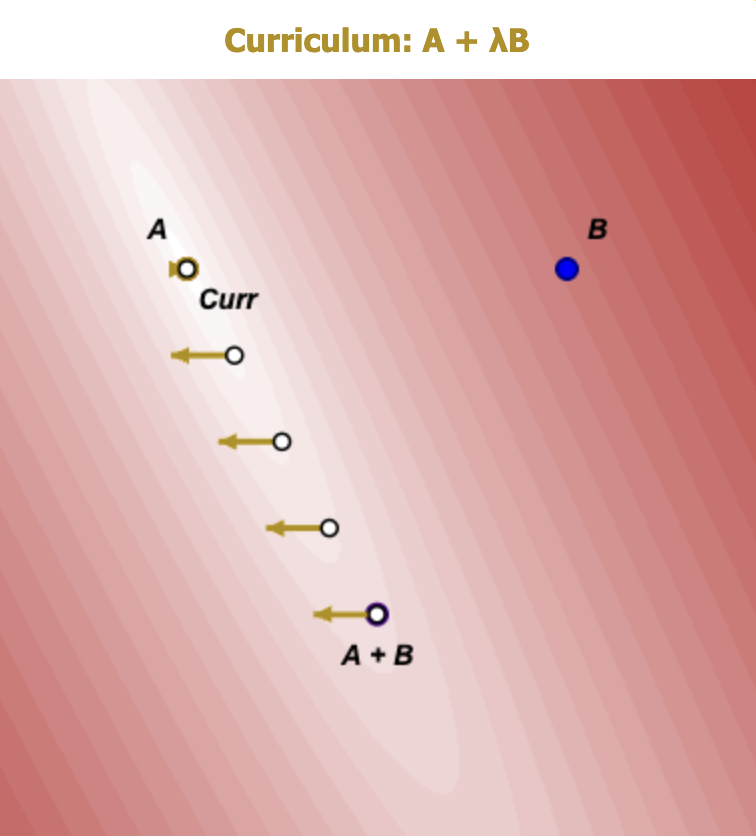
\includegraphics[width=\linewidth]{img/joint_loss_lambda_evolution/joint_loss_lambda_0.png}\\
        {\scriptsize $\lambda = 0$}
    \end{minipage}\hfill
    \begin{minipage}[t]{0.31\linewidth}\centering
        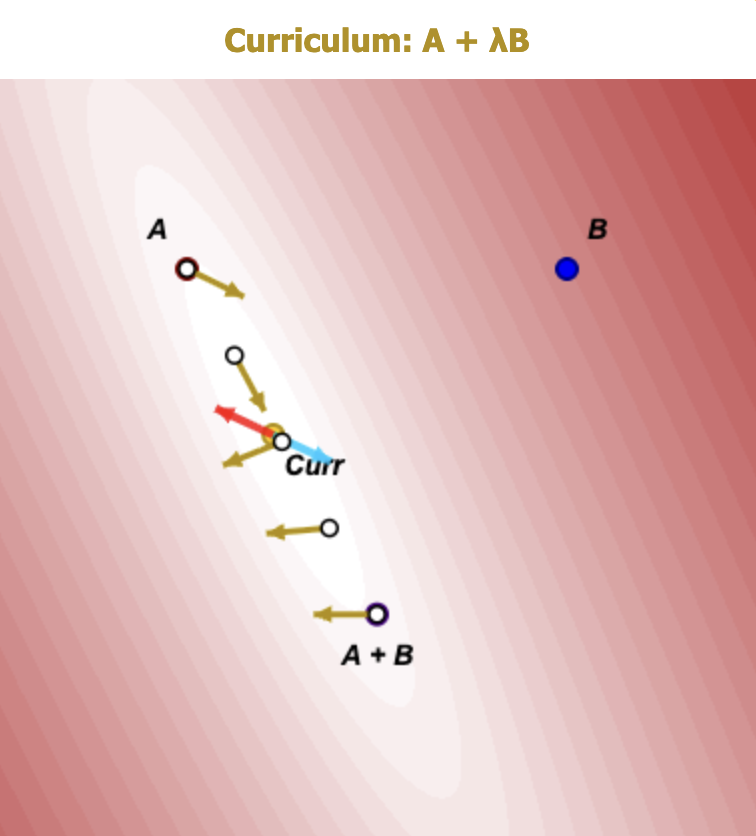
\includegraphics[width=\linewidth]{img/joint_loss_lambda_evolution/joint_loss_lambda_0_025.png}\\
        {\scriptsize $\lambda = 0.025$}
    \end{minipage}\hfill
    \begin{minipage}[t]{0.31\linewidth}\centering
        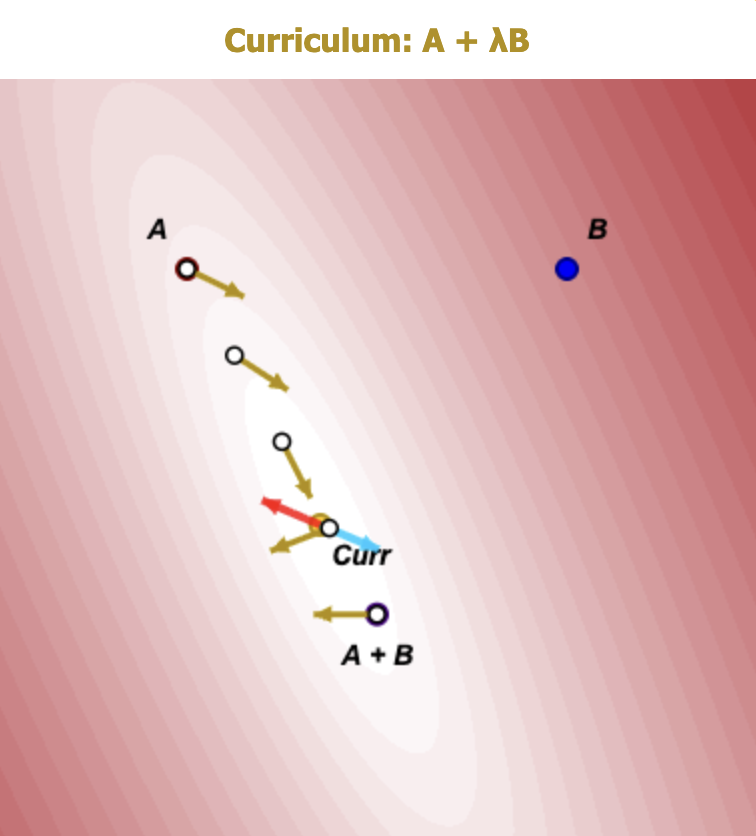
\includegraphics[width=\linewidth]{img/joint_loss_lambda_evolution/joint_loss_lambda_0_07.png}\\
        {\scriptsize $\lambda = 0.07$}
    \end{minipage}

    \vspace{0.5em}
    \begin{minipage}[t]{0.31\linewidth}\centering
        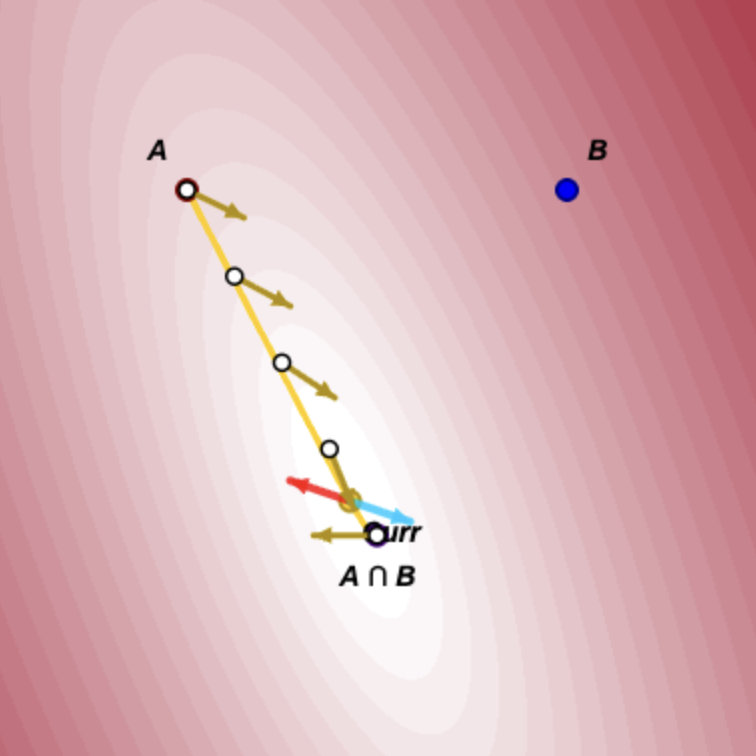
\includegraphics[width=\linewidth]{img/joint_loss_lambda_evolution/joint_loss_lambda_0_175.png}\\
        {\scriptsize $\lambda = 0.175$}
    \end{minipage}\hfill
    \begin{minipage}[t]{0.31\linewidth}\centering
        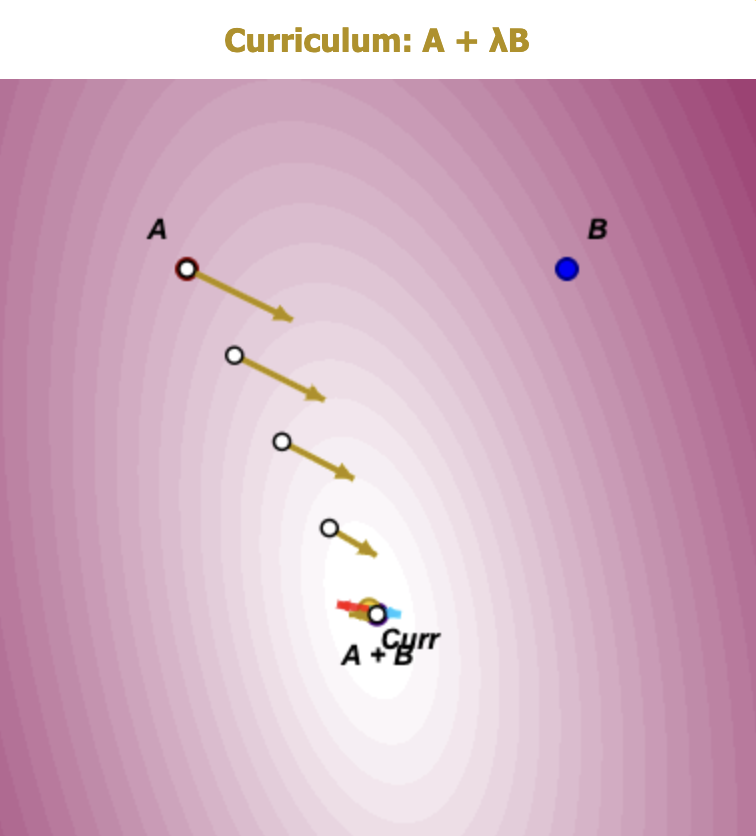
\includegraphics[width=\linewidth]{img/joint_loss_lambda_evolution/joint_loss_lambda_0_5.png}\\
        {\scriptsize $\lambda = 0.5$}
    \end{minipage}\hfill
    \begin{minipage}[t]{0.31\linewidth}\centering
        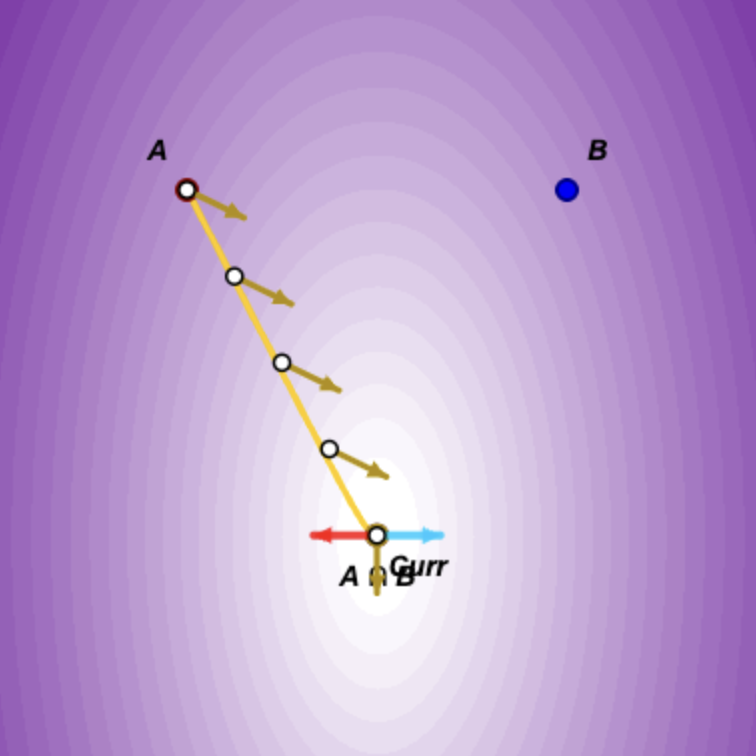
\includegraphics[width=\linewidth]{img/joint_loss_lambda_evolution/joint_loss_lambda_1.png}\\
        {\scriptsize $\lambda = 1$}
    \end{minipage}

    \caption{Evolution of the curriculum loss $L_\lambda = A + \lambda B$. As $\lambda$ increases, the contours morph continuously from the old-task basin around $A$ to the joint basin around $A{+}B$. The current minimiser (\emph{Curr}) slides along the moving valley floor, forming the reference path $\Theta^*(\lambda)$. At the minimiser, the replay (red) and current-task (blue) gradients cancel; the joint gradient (golden) vanishes at the minimiser and points down the valley, ensuring a tracking model rides the floor instead of teleporting across the landscape.}
    \label{fig:lambda_evolution}
\end{figure}

\subsection{The Two-Level Gap: Bowing and Overshoot}
\label{subsec:trajectory_problem}

Real trajectories deviate from the reference path on two distinct levels.\\

\textbf{Level One (The Bow):} Even under highly idealised conditions (exact gradients, vanishing step size), the steepest-descent direction of the abruptly assembled joint loss misaligns with the direction toward the joint minimum whenever the loss curves more sharply in some directions than in others. The trajectory bows outward, leaving the old task's basin before returning \citep{kao2021naturalcontinuallearningsuccess}. This deterministic out-and-back arc forms the structural core of the gap (Figure~\ref{fig:loss_landscape_visualization}, green curve).\\

\textbf{Level Two (Overshoot):} Real training dynamics inflate this arc. At a sudden task boundary, the minimum teleports from $\theta_A^*$ to $\theta_{\text{joint}}^*$, leaving the iterate exposed to a large new-task gradient while the replay gradient is near zero \citep{delange2023continualevaluationlifelonglearning}. Two acute drivers, finite step sizes and momentum accumulation, amplify this unopposed push, creating the sharp first-step drop. Concurrently, a chronic driver, estimator variance from finite buffer sampling (Section~\ref{subsec:experience_replay}), injects noise that delays the slow recovery tail.\\

\textbf{The Tracking Bound:} Stretching the transition over an $N$-step ramp resolves both levels at once. Introducing the new task slowly ($\lambda \approx 1/N$) makes the reference path of Section~\ref{subsec:reference} the path the dynamics actually define, so the bow disappears; and it keeps the iterate tethered to the moving valley floor $\Theta^*(\lambda(t))$ rather than leaping across the landscape, with a tracking lag that a gradient-flow analysis bounds by $O(1/N)$ (Appendix~\ref{app:detailed_proof}). The two combine to cap the highest transient replay loss during the transition:
\begin{equation}
    \max_t\, L_{\text{replay}}(\theta(t)) \;\le\; L_{\text{replay}}(\theta_{\text{joint}}^*) + O\!\left(\frac{1}{N}\right),
    \label{eq:bound}
\end{equation}
where the first term is the permanent price of Section~\ref{subsec:reference} and the second is the transient, which shrinks with ramp length. This continuous-limit argument controls the deterministic arc and the acute overshoot, but the per-step stochastic noise of the buffer survives any ramp length and requires a separate remedy, addressed in the momentum experiments of Section~\ref{subsec:momentum}.

The two levels partition the gap's two dimensions: the acute drivers set the depth of the initial drop, while the hanging tail is the Level-One arc plus the slow, noisy recovery the chronic driver leaves behind. This yields the falsifiable core tested as RQ1: removing the overshoot drivers should flatten the drop and leave the arc, placing the optimiser on the reference path should remove the arc and leave the overshoot, and doing both should close the gap while the permanent cost of Section~\ref{subsec:reference} remains.

\subsection{Two Gates: Attenuating the New-Task Gradient}
\label{subsec:gates}

Equation~\eqref{eq:unified_update} shows that replay methods differ mainly in how they weight the replay and current-task gradients. The replay gradient is the only restoring force pulling the iterate back to the reference path, so a protective method must attenuate the new-task push---the source of the bow and overshoot---while leaving the restoring gradient intact. Generalising the current-task weight to an operator $G$ yields a one-sided \emph{gate}:
\begin{equation}
    d \;=\; G\, g_{\text{cur}} \;+\; g_{\text{rep}}.
    \label{eq:gate}
\end{equation}

The curriculum of Section~\ref{subsec:reference} realises this gate along one axis, \emph{time}: it introduces the new task slowly, so the push is never large enough at once to knock the iterate off the reference path. A complementary axis is \emph{direction}. At any single step only part of the push is harmful, because the past task is flat in most directions and steeply curved in a few, and only motion along the steep directions raises the replay loss. Preconditioning the push by past-task curvature exploits this, passing it at full gain where the past task is flat and shrinking it where the past task is steep, so retention costs little plasticity. This natural-gradient idea underlies Natural Continual Learning \citep{kao2021naturalcontinuallearningsuccess} and, in a replay setting, Online Curvature-Aware Replay \citep{urettini2025onlinecurvatureawarereplay}. Both, however, precondition the \emph{entire} update, so the same metric that brakes the harmful push also brakes the restoring replay gradient---protecting the past task only by slowing the return to it. Asymmetric PER keeps the gate one-sided: it filters the new-task gradient alone and leaves the restoring gradient at full strength. We include the symmetric preconditioner, which damps both, as a control (Appendix~\ref{app:per_sym}).

As detailed in Table~\ref{tab:gates}, gates vary by their \emph{domain} (scalar vs.\ directional) and \emph{control} (feedback vs.\ feedforward). This thesis explores the two pure corners of this design space:

\begin{description}
    \item[Adaptive $\lambda$-curriculum (Scalar Feedback):] A scheduling parameter $\lambda(t)$ sets the new-task weight from the ratio of replay to new-task gradient norms. By scaling the loss itself, it deforms the objective into the homotopy of Section~\ref{subsec:reference}, so the optimiser's natural descent follows the reference path.
    \item[Asymmetric PER (Directional Feedforward):] The gate $G = \delta(F_{\text{rep}}+\delta I)^{-1}$ is a fixed filter set by the replay Fisher, with the damping $\delta$ its single knob: as $\delta \to 0$ the push concentrates in the directions the past task is flat in. Committed in advance, it is feedforward, and therefore blind to damage arriving from directions the sampled Fisher misreads.
\end{description}

\begin{table}[htbp]
    \centering
    \small
    \resizebox{\columnwidth}{!}{%
        \begin{tabular}{@{}l l l l@{}}
            \hline
            Method           & Gate $G$                               & Domain      & Control     \\
            \hline
            Vanilla ER       & $I$                                    & ---         & ---         \\
            GEM / A-GEM      & reweight on conflict                   & scalar      & feedback    \\
            MEGA             & loss ratio                             & scalar      & feedback    \\
            Balancing        & norm matching                          & scalar      & feedback    \\
            Linear curric.   & $\lambda(t)\,I$, clock                 & scalar      & feedforward \\
            Adaptive curric. & $\lambda(t)\,I$, norm ratio            & scalar      & feedback    \\
            Asym.\ PER       & $\delta(F_{\text{rep}}+\delta I)^{-1}$ & directional & feedforward \\
            \hline
        \end{tabular}%
    }
    \caption{Replay methods as gates on the new-task gradient, Equation~\eqref{eq:gate}. The two methods of this thesis occupy the pure corners: a scalar feedback gate and a directional feedforward gate.}
    \label{tab:gates}
\end{table}



% \section{The Stability Gap as a Trajectory Problem}
% \label{sec:motivation}
% This section develops the two-level account. Learning a new task permanently moves the model, and part of the past-task loss it gives up is the price of that move; the stability gap is the extra loss on top, a dip below the settled level followed by recovery. That excess has two sources: a geometric detour that bows even an ideal optimiser's path, and a preventable overshoot that real training adds. The subsections make each precise, then show that one design choice, how the update treats the new-task gradient, governs both and organises the methods of this thesis.

% \subsection{The Permanent Cost and the Reference Path}
% \label{subsec:reference}

% Learning a second task moves the model. In a quadratic picture with task losses $L_A$ and $L_B$ and Hessians $H_A$ and $H_B$, the joint minimum sits at displacement $\theta_{\text{joint}}^* - \theta_A^* = (H_A+H_B)^{-1}H_B\,(\theta_B^*-\theta_A^*)$ from the old optimum, and the replay loss ends higher by approximately $\tfrac{1}{2}\,d^\top H_A\, d$ for that displacement $d$. This rise is the permanent stability--plasticity price. Every method pays it, and it is distinct from the stability gap.

% The rise can be monotone. Consider the family of objectives $L_\lambda = L_{\text{replay}} + \lambda L_{\text{current}}$ and the path $\Theta^*(\lambda)$ traced by its minimiser as $\lambda$ grows from $0$ to $1$. Section~\ref{sec:theory} shows, with an envelope-theorem argument, that the replay loss increases monotonically along this path under a local positive-definiteness condition. The path starts at $\theta_A^*$, ends at $\theta_{\text{joint}}^*$, and the replay loss climbs directly to its final level with no excursion above it. We call $\Theta^*(\lambda)$ the \emph{reference path}. Mode connectivity gives the empirical counterpart: low-loss routes between the sequential and joint solutions exist in trained networks (Section~\ref{subsec:lmc}).

% The reference path defines the gap. Everything the past-task loss does \emph{above its eventual settled level, and back}, exceeds what learning the new task requires. The stability gap is exactly this transient excess: a dip below the settled accuracy level followed by recovery.

% \subsection{Level One: the Path Bows}
% \label{subsec:trajectory_problem}
% Take the most idealised optimiser available: exact gradients and vanishing step size, pure gradient flow on the joint loss, started at $\theta_A^*$ the moment the task switches. Its path still deviates from the reference. The steepest-descent direction of the joint loss and the direction toward the joint minimum disagree whenever the loss is more steeply curved in some directions than in others, so the flow bows outward, leaves the old task's basin, crosses a region of higher replay loss, and approaches the joint minimum from outside \citep{kao2021naturalcontinuallearningsuccess}. Along this bow the replay loss rises above its final level and returns, an out-and-back \emph{arc}. Figure~\ref{fig:loss_landscape_visualization} draws it as the green curve.

% The arc is the structural core of the gap, for three reasons. It is deterministic: gradient noise, learning rate, and momentum play no role in it, so it survives exact replay gradients and careful step sizes. It explains the persistence results of Section~\ref{subsec:stability_gap}: a perfect objective changes which surface is descended, but leaves the descent direction, and with it the bow, in place. And its cost scales with recovery time: the arc shows up as a dip that stays open while the iterate walks around the bow, so it dominates on networks that reconverge slowly. Fixing the arc requires changing which path the dynamics define; following the bowed path more carefully leaves it untouched.

% \subsection{Level Two: Overshoot of the Followed Path}
% \label{subsec:overshoot}

% Level One held the optimiser to an ideal: exact gradients, vanishing steps, no momentum. Real training meets none of these conditions, and each departure pushes the iterate beyond the path its own dynamics define, adding overshoot on top of the bow. Three mechanisms drive this overshoot, and they differ in when they act. Two are acute, set off by the task boundary. When the task switches, the objective jumps in one step from the replay loss to the joint loss, so the minimum the parameters chase teleports from $\theta_A^*$ to $\theta_{\text{joint}}^*$ while the parameters stand still. The iterate is left where the replay gradient is near zero, by convergence on Task A, and where the new-task gradient is at its largest, because Task B is unlearned \citep{delange2023continualevaluationlifelonglearning}. This lopsided push, strongest in the first steps after the switch, is what the two acute drivers exploit. The third driver is chronic. It comes from replaying a finite buffer, is present at every step rather than triggered by the switch, and feeds the slow tail rather than the sharp drop.

% \begin{description}
%     \item[Imbalance $\times$ step size (acute).] With a finite learning rate, the first discrete steps ride the unopposed new-task gradient far past where the trajectory would be, a single large leap out of the old basin with a steep recovery once the replay loss kicks in. This is the mechanism behind the sharp first-step drop.
%     \item[Momentum accumulation (acute).] Momentum accumulates the sustained early push toward roughly $1/(1-\beta)$ times its per-step size. At the boundary the sustained direction is the provisional, old-task-degrading one, so the amplification lands exactly where it hurts.
%     \item[Estimator variance (chronic).] The buffer gradient is a noisy version of the true past-task gradient (Section~\ref{subsec:experience_replay}), and it stays noisy for the whole task rather than only at the switch. Noise in the restoring force lets the iterate wander off the path and settle back slowly, so its mark is a lingering residual and a slow, jittery recovery rather than the first-step drop.
% \end{description}

% Two properties matter. First, the drivers interact: the displacement grows roughly with the size of the push, the number of steps before the restoring gradient bites, and the amplification on top, with noise jittering the whole excursion. They are mechanisms of one process, and their contributions resist clean separation into additive shares. Second, overshoot is path-agnostic: it inflates the arc of the bowed path, and it is the entire residual transient around the reference path once the arc is gone.

% The two levels also assign the gap's two dimensions. The depth of the drop is set by the acute drivers; the hanging tail is the arc of Level One plus the slow, noisy recovery left by the chronic driver. This yields the falsifiable core of the thesis, tested as RQ1: removing the overshoot drivers should flatten the drop and leave the arc; placing the optimiser on the reference path should remove the arc and leave the overshoot; doing both should remove the gap while the permanent cost of Section~\ref{subsec:reference} remains.

% \subsection{Two Gates}
% \label{subsec:gates}
% The unified update of Equation~\eqref{eq:unified_update} shows that replay methods differ only in how they weight the two gradients. One asymmetry in the problem dictates how the weights should be used. The replay gradient is the only force pulling the iterate back toward the reference path, so attenuating it works against retention; the new-task gradient is the source of both the bow and the overshoot, so attenuation belongs there. Generalising the current-task weight from a scalar to an operator $G$ gives the shared form
% \begin{equation}
%     d \;=\; G\, g_{\text{cur}} \;+\; g_{\text{rep}},
%     \label{eq:gate}
% \end{equation}
% a \emph{gate} on the new-task push with the restoring force at full strength. A symmetric alternative would filter the whole update through past-task curvature, braking the restoring force as hard as the harmful push. But the restoring force is exactly what pulls the model back onto the reference path, so braking both at once protects the past task only by stalling the model. The gate must therefore be one-sided: hold back the new-task push and leave the restoring force untouched.

% Every method of Section~\ref{subsec:path_finding} instantiates Equation~\eqref{eq:gate}, and two design axes span the family. The gate's \emph{domain} is scalar or directional: a scalar gate attenuates the whole push, so protection is paid in plasticity, while a directional gate attenuates per direction, passing the push where the past task is flat and braking it where the past task is steep, protection nearly for free when the metric is right. The gate's \emph{control} is feedback or feedforward: a feedback gate reads a live damage signal and reacts to harm from any direction, while a feedforward gate commits to a schedule or a precomputed filter and is only as good as its model of where harm lives.

% The two methods of this thesis are the pure corners. The \textbf{adaptive $\lambda$-curriculum} is the scalar feedback gate: $\lambda(t)$ rises with the ratio of replay to new-task gradient norms, a signal that fires whichever direction damage arrives from. Because $\lambda$ scales the loss itself, the gate deforms the objective into the homotopy of Section~\ref{subsec:reference}: it schedules the landscape so that the route the optimiser naturally takes is the reference path. \textbf{Asymmetric PER} is the directional feedforward gate: it filters the push through the replay Fisher, Equation~\eqref{eq:asym_per}, with the damping $\delta$ as its single knob. At $\delta \to \infty$ the filter opens fully and plain ER returns; at $\delta \to 0$ motion concentrates in directions the past task is flat in, while restoration keeps full strength. Table~\ref{tab:gates} places the replay methods on the two axes and marks where each corner sits.

% \begin{table}[htbp]
%     \centering
%     \small
%     \resizebox{\columnwidth}{!}{%
%         \begin{tabular}{@{}l l l l@{}}
%             \hline
%             Method           & Gate $G$                               & Domain      & Control     \\
%             \hline
%             Vanilla ER       & $I$                                    & ---         & ---         \\
%             GEM / A-GEM      & reweight on conflict                   & scalar      & feedback    \\
%             MEGA             & loss ratio                             & scalar      & feedback    \\
%             Balancing        & norm matching                          & scalar      & feedback    \\
%             Linear curric.   & $\lambda(t)\,I$, clock                 & scalar      & feedforward \\
%             Adaptive curric. & $\lambda(t)\,I$, norm ratio            & scalar      & feedback    \\
%             Asym.\ PER       & $\delta(F_{\text{rep}}+\delta I)^{-1}$ & directional & feedforward \\
%             \hline
%         \end{tabular}%
%     }
%     \caption{Replay methods as gates on the new-task gradient, Equation~\eqref{eq:gate}. The two methods of this thesis occupy the pure corners: a scalar feedback gate and a directional feedforward gate.}
%     \label{tab:gates}
% \end{table}

% The taxonomy yields testable hypotheses that Section~\ref{sec:proposed_approach} formalises as research questions. The scalar feedback gate is hard to blind-side but slows the new task everywhere, so it should pay a plasticity cost a separate accelerator must repay. The directional gate should protect the past task at little plasticity cost, but only within what its sampled curvature metric sees. The two should interact oppositely with momentum: the curriculum attenuates \emph{at source}, so with $\lambda \approx 0$ early there is nothing to accumulate and acceleration helps, whereas the preconditioner attenuates each \emph{step} while the gradient keeps its size, so accumulation across steps can rebuild the push the filter removed and momentum should partly undo the protection.
